%\vspace*{-0.3cm}
\subsection{Simulation Evaluation}
\label{subsec:eval-sim}


  \begin{figure}
  \centering
  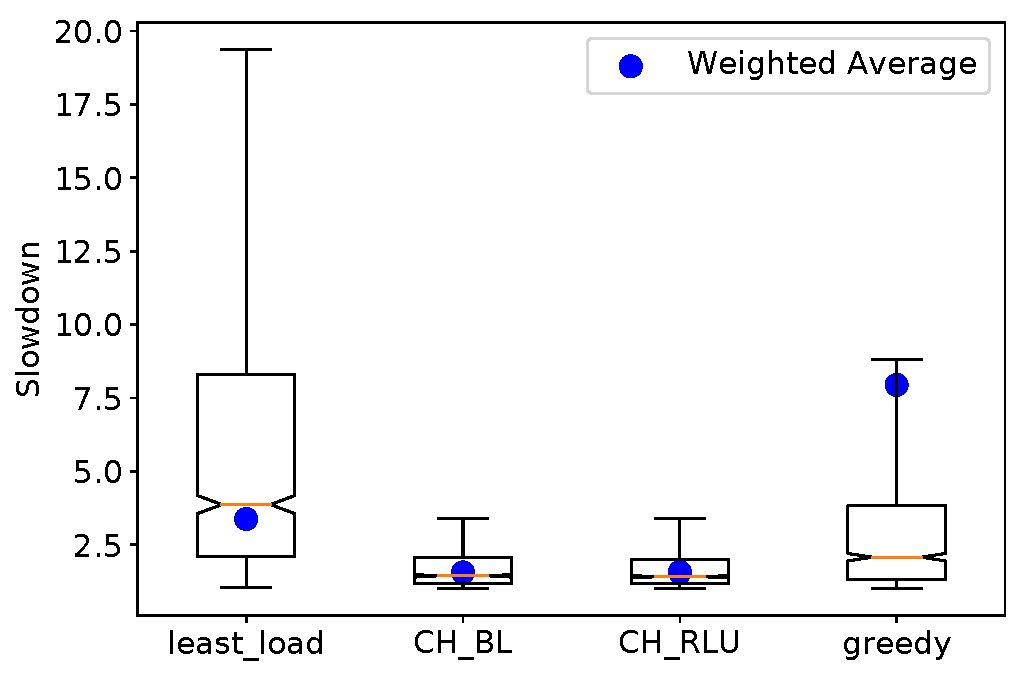
\includegraphics[width=0.3\textwidth]{chrlu/faaslb-osdi22/figs/1k/latencies-GD.pdf}
%  \vspace*{-0.3cm}
  \caption{[Simulated] Function latency distribution. }
  \label{fig:1k-lat}
%  \vspace*{-0.3cm}
  \end{figure}

\begin{figure}
  \centering
  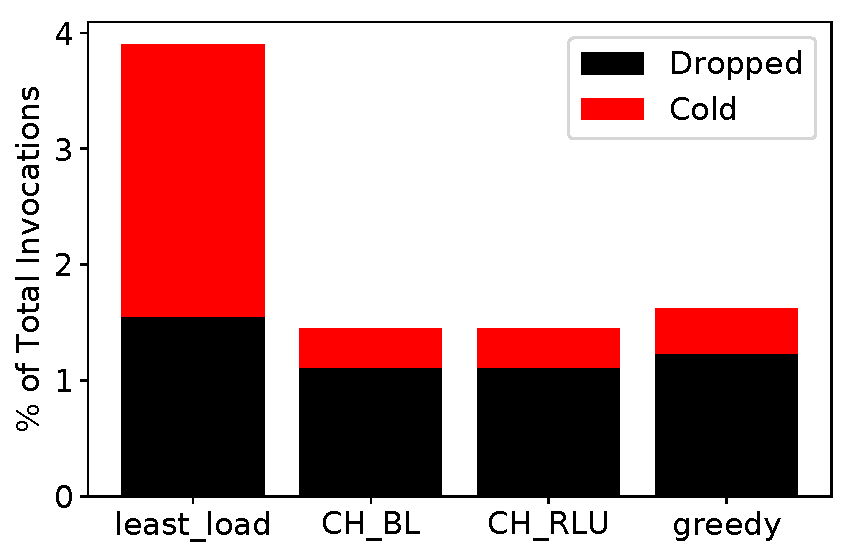
\includegraphics[width=0.3\textwidth]{chrlu/faaslb-osdi22/figs/1k/cd-GD.pdf}
%    \vspace*{-0.3cm}
  \caption{[Simulated] Cold and dropped functions.}
  \label{fig:1k-cd}
%    \vspace*{-0.3cm}
\end{figure}


To investigate the performance of various load-balancing policies at larger scales, we use a simulation approach.
We have developed a discrete-event simulator, which plays a function workload trace, and emulates the various aspects of function execution and slowdown: slow/warm starts, slowdown due to concurrent processing by emulating a G/G/k queuing system on each server, and various load metrics (emulating Linux exponentially decaying load averages, stale loads, real-time loads, etc.). 
The simulator allows us to implement different policies using information that would not otherwise be available on a real system: accurate function cold and warm times, instant load information, etc.
The function running times are computed by adding the actual provider-captured running times to the OpenWhisk and Docker startup overheads that are empirically measured and modeled.
This, when combined with queuing delays, captures the overall slowdown due to concurrent processing.
The simulator is implemented in Python in about 3,000 lines of code. 

We run the Azure trace with 1000 randomly chosen functions spanning almost a million invocations, and compare different load-balancing policies.
This workload is highly bursty and is characterized by the Figures in Section~\ref{sec:challenges}. 
We have implemented a ``online greedy optimal'' policy that considers \emph{all} servers when running functions, by picking the server with the lowest expected running time (based on Section~\ref{subsec:chch}).
This would be impractical and unrealistic to implement, since it needs accurate information about every function's keep-alive status on every server, and an accurate model of function performance at various loads.
Nevertheless, it provides an optimistic baseline: our consistent-hashing based policy ($CH-RLU$) is significantly simpler, only considers a small subset of servers, and does not require omniscient cluster state. 

Figure~\ref{fig:1k-lat} compares this greedy policy with a locality-agnostic ``least-loaded'' policy that is popular in web-clusters, and the two consistent-hashing based policies. 
The figure shows the function slowdown factor for each function, as well as the global average slowdown.
Slowdown is defined as the ratio of function's execution time to its base warm time without any system overhead, resource contention, or queuing delays.
Most functions do poorly with the least-loaded policy: the median function slowdown is almost $4\times$, primarily because of high cold starts.
Figure~\ref{fig:1k-cd} compares the cold and dropped statistics for the various policies.

Returning to Figure~\ref{fig:1k-lat}, both CH-BL and CH-RLU have comparable performance, with a median slowdown of $2.4$. 
Finally, and surprisingly, the omniscient greedy policy performs poorly: with the global slowdown approaching $7$.
The primary reason for this is because of the bursty nature of the workload: the greedy policy tends to pick the server with the least-loaded server that can run the warm function.
However because of stale load information, we see a \emph{herd effect} on the server, and this causes extremely high resource contention and latency, even though the number of cold starts is small (compared in Figure~\ref{fig:1k-cd}). 


% \begin{centering}
\begin{figure}
  \centering
  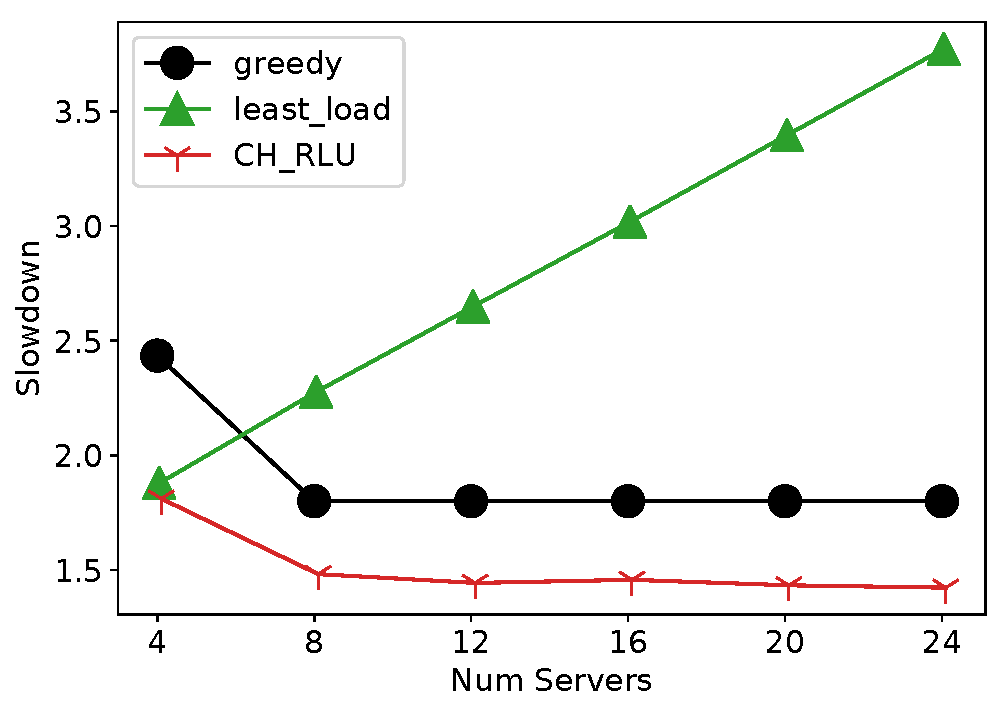
\includegraphics[width=0.3\textwidth]{chrlu/faaslb-osdi22/figs/1k/latencies-250scaling.pdf}
  %  \vspace*{-0.3cm}
  \caption{[Simulated] Function latencies as cluster size is increased. Least-loaded performs \emph{worse} because its locality and cold starts become worse as more servers are added.}
  \label{fig:1k-scaling}
 %   \vspace*{-0.3cm}
\end{figure}
% \end{centering}

Finally, we investigate performance when the cluster size changes.
Figure~\ref{fig:1k-scaling} shows the slowdown for the three policies when the number of servers is increased.
Importantly, the total number of computing and memory in the cluster is kept constant at 256 CPUs and 512 GB, and the size of the individual servers is changed.
Thus 4 servers with 64 CPUs are compared with 8 servers with 32 CPUs, etc.
This experiment is intended to capture the effects of locality: smaller number of servers may have a higher hit-rate, and a more even load-spread.

Figure~\ref{fig:1k-scaling} shows how the function slowdown for both CH-RLU and greedy decays as the number of servers is increased.  
This is because larger servers see heavier lock and other resource contention, and thus while they may exhibit better locality, the load-induced slowdown dominates.
This has important ramifications for large FaaS providers, since they can continue using smaller servers for running functions, and expands the utility of small deflatable/harvestable VMs for running colocated functions~\cite{serverless-harvest-sosp21}.

CH-RLU reduces the function slowdown by 20\% compared to the greedy approach, across a wide range of cluster configurations in Figure~\ref{fig:1k-scaling}. 
Interestingly, least-loaded's performance worsens with increasing number of servers and fragmentation.
The main culprit is worsening locality.
With a small number of servers, least-loaded can get ``lucky'' and score a keep-alive cache-hit.
These fortuitous warm-starts get less probable with an increasing number of servers. 

%%% Local Variables:
%%% mode: latex
%%% TeX-master: "paper"
%%% End:

